\section{Functional Role of Remixing}

The previous section helped describe the structural properties of the Scratch Online Community as a remixing system.
This section is intended to examine what people do.
In particular, the goal is to understand what are the various roles that remixing plays and how it is part of collaborative and creative practices.

Remixing represents many activities in Scratch.
For example, people occasionally remix to fix software bugs on someone's project, in other cases people want to add to an existing project to customize it or make it more personal, in others, people want to start a trend or ``meme'' so they create a ``template'' project just so others remix it, add to it and pass it on.

To map these varied types of remixing, based on previous analysis of other remixing online communities \citep{seneviratne_remix_2010}, I focus on two dimensions:
\begin{enumerate}
\item{Similarity}. This indicates how different a remix is from the original work on which it is based. 
Remixes can range from merely being inspired by someone's idea, to tweaking someone's project, to making an exact copy.
This is an important aspect of remixing because it gets at the core of some of the tensions around remixing, and it also helps us understand the degree of interaction and creative output between a remix and its antecedent project.
\item{Number of people}. This indicates the number people involved or intended to be involved in the remix.
Remixes can range from a single author (for example, a creator remixing herself as a form of version control), to a small group of people (for example, a team collaborating in making projects), to a crowd (for example, a large group of people participating in a remix chain).
The number of people involved is a useful dimension because it helps us identify the distinct roles remixing plays in Scratch.
\end{enumerate}

Using these two dimensions, one can identify a set of remixing categories (Figure~\ref{fig:function} useful for the analysis of the functional roles of remixing in Scratch.
Broadly speaking, the types of remixing I plan to use to guide my analyses are the following:

\begin{figure}
\centering
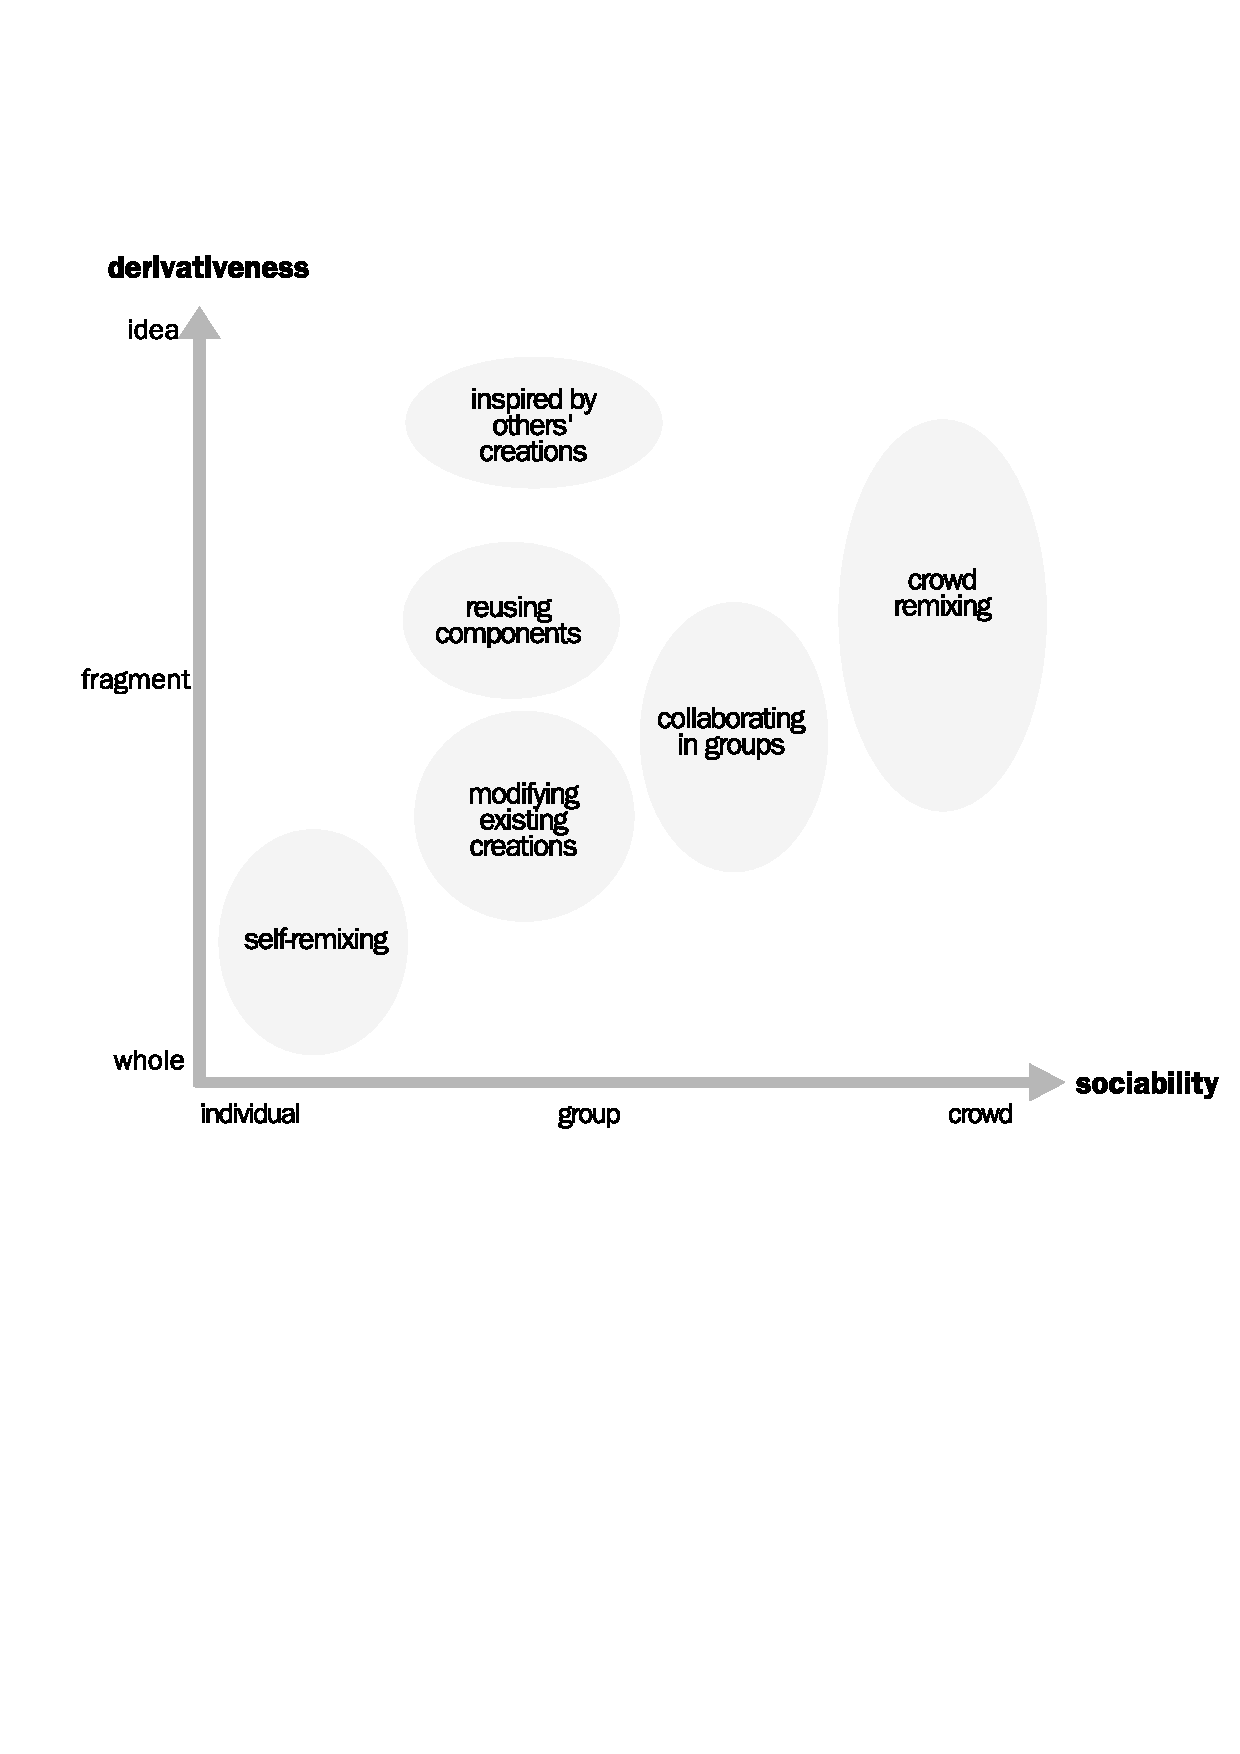
\includegraphics[width=3.25in]{figures/function.pdf}
\caption{Functional roles of remixing in the social and product-focus dimensions}
\label{fig:function}
\end{figure}

\subsection{Incremental Remixing}
This type of remixing often involves downloading someone's project to customize it or to fix a bug. 
For example, replacing the costumes of a sprite in a game for a different one. 
This form of remixing often occurs when people make small modifications to the sample projects that come preinstalled with Scratch.
Also anecdotal evidence suggests that this form of remixing tends to be a useful way for newcomers to get started with Scratch,  modifying an existing project instead of creating a completely new project.
This type of remixing sometimes leads to controversy when the changes are subtle or nonexistent.
Project creators sometimes argue that types of remixing in which the changes are minimal should not be allowed.

\subsection{Component Remixing}
Remixing also occurs when people use pieces of others' projects to produce something new, rather than building on top of existing work.   
In these cases, often one cannot quickly tell in what way the remix and the original are related.
This type of remixing typically involves some sample sprites that come preinstalled with Scratch, such as the ``jetpack girl'' example mentioned above or some of the templates, images or sounds that members of the community explicitly created for others to reuse.


\subsection{Group Remixing}
Remixing is also used by groups or ``collabs'', as they are often referred to by Scratch members, to work collaboratively by remixing one another's work almost aform of version control \citep{tichy_rcs_1985}.
For example, we found in that one of the ``collabs'' we analyzed, one member of the group would start by creating a first version of the project they had decided to make while others would work on varied parts such as the images, sounds or the engine of a game \citep{aragon_tale_2009}, .
In that particular ``collab'' there were, on average, seventeen remixes before officially releasing a project.
In this case, remixing is part of an explicit collaborative activity.


\subsection{Crowd Remixing}
The home page of the Scratch website has a section called ``What the Community is Remixing''  that features the three top remixed projects in the past two weeks.
Although these projects could represent any type of remixing, they are typically projects that consist of a compelling template that encourages people to add something small to it and pass it on to someone else, like a chain.
For example, one of those projects titled ``Add yourself to the party'' shows a character dancing on a colorful dance floor by itself.
The creator leaves a note in the description of the project inviting people to download the project and add a sprite representing their avatar or profile picture.
Other examples are ``Remix if you care about animal rights'', representing a type of crowd remixing with a social cause, and ``Coloring contest'', representing popular genre among more artistic-inclined community members that consists of downloading a still image (often with music playing in the background), coloring it and submitting it to a contest for the best-colored image.
Although typically the intention of the creator of this type of project is to create a chain, often the structure of the remix network looks more like a star because of people not following the rules or not checking where the last element of the chain is.
These types of remixes are often incremental like the category described above, but the relationship between the creator and its intended audience is significantly different. 
Crowd remixing explicitly invites people to remix en masse following a specific template. 
The purpose of the creation is not the creation itself but the collection of many remixes created by many individuals.
Evidence suggests that this type of crowd remixing emerged after the top remixed projects section was added to the website, but more research is needed to understand these phenomena.

\subsection{Inspirational Remixing}
On the far end of the similarity spectrum are projects that are projects inspired by other projects that do not use any particular component of the original work.
These projects are often trying to replicate popular software, video games or even genres that have emerged in the community.
For example, some people create remixes of the Microsoft Windows operating system, or the iPhone, or operating systems that other members of the community have created such as SynOS, a popular Scratch-based pseudo-operating system created by a teenage member of the community.
Other examples of inspirational remixes are the ``fan art'' projects created after popular characters created by other members of the Scratch community such as ``Maki-Tak'', a lizard that dances and sings in animations created by a teenage girl,  or  ``Mr. Happy Man'', a grumpy character invented by a teenage boy.
This type of inspirational remixing is a lot harder to identify automatically because the original and the remix do not share any bytes but their names, descriptions and log data might help. 

\subsection{Self-remixing}
%  TODO: Check this number.
About 13\% of remixes are projects created based on the same person's projects.
This is typically used as some form of version control.
For example, sometimes children create a Scratch project at school, upload it to the website, download it at home, continue working on it, then re-upload it to the website under a name like ``My video game v2''.
When this happens, the website identifies them as remixes and links them back to their previous version.
A few people, mainly popular Scratch creators who care about the projects displayed on their profile page, have two accounts: one for testing and one for sharing final version of their projects.
For example, there is an adult member of the community who has two usernames: ``Paddle2See'' and ``Paddle2SeeTest''.
As the name implies, one is often used for sharing drafts or work in progress.
 
\subsection{Proposed work}
In this section of my dissertation I plan to describe the way people engage in remixing on the Scratch Online Community. 
In particular, I plan to answer questions such as:
1. Are the types of remixing described above representative for Scratch and generalizable for other online remixing communities? 
For this, I plan to connect with other researchers investigating other online communities, especially ccMixter.org.
2. What kind of people engage in each type of remixing? For example, do novices engage in incremental and crowd remixing more often than component remixing? Are the originators of crowd remixing longtime members of the community and how do they manage to get more people to remix their work?
3. In what way does each type of remixing help scaffold Scratch participation? For example, are some types of remixing better at learning the technical aspects of Scratch while others are more helpful in learning how to collaborate and socialize online? Are people who engage in remixing initially more likely to stay active on the community and in what ways?
4. How have these types of remixing evolved over the course of three years?
Are the social networks created through various types of remixing different in their structure and quality?
5. How do the projects in each type of remixing differ technically and in content? For example, in what ways might some types be more complex than others?
The distinctions amongst the types are subjective at this point, and part of the work I plan to do is to clearly identify the boundaries among categories.

